Qui, di seguito, viene riportata l'architettura relativa alla quinta solution.

\lstinputlisting[language=C++]{solutions/s5/s5.cpp}

In particolare, nella soluzione hardware in questione, rispetto alla solution 2 dove era presenta solo la direttiva di unrolling nel loop2,, è stata aggiunta la direttiva di unrolling con fattore pari a 2 all'interno del loop2.

Effettuando la sintesi è possibile evidenziare il seguente report:\\

\begin{table}[H]
	\centering
	\begin{minipage}[t]{0.45\linewidth}
		\centering
		\begin{tabular}{|c|c|c|c|}
			\hline
			\textbf{Clock} & \textbf{Target} & \textbf{Estimated} & \textbf{Uncertainty} \\
			\hline
			ap\_clk & 10.00 & 8.510 & 1.25 \\
			\hline
		\end{tabular}
		\caption{HLS Solution 5 Timing Summary (ns)}
		\label{tab:hls-solution-5-timing-summary}
	\end{minipage}
	\hfill
	\begin{minipage}[t]{0.45\linewidth}
		\centering
		\begin{tabular}{|c|c|c|c|}
			\hline
			\multicolumn{2}{|c|}{\textbf{Latency}} & \multicolumn{2}{|c|}{\textbf{Interval}} \\
			min & max & min & max \\
			\hline
			33 & 41 & 33 & 41 \\
			\hline
		\end{tabular}
		\caption{HLS Solution 5 Latency Summary (clock cycles)}
		\label{tab:hls-solution-5-latency-summary}
	\end{minipage}
\end{table}

In particolare, si può notare come, rispetto alla solution 2 dove il trip count relativo al loop2 era pari a $0\sim4$, in questo caso il trip count associato al loop2 risulta essere dimezzato dal momento che è stato previsto un unrolling di fattore pari a 2 all'interno del ciclo in questione. Inoltre, dal momento che è stato introdotto una direttiva di pipeline all'interno del loop2, si può evidenziare come l'Initiation Interval raggiunto risulta essere il medesimo di quello target.

\begin{table}[H]
	\centering
	\begin{tabular}{|c|c|c|c|c|c|c|c|c|}
		\hline
		\multicolumn{1}{|c|}{Loop} & \multicolumn{2}{|c|}{\textbf{Latency}} & \multicolumn{1}{c|}{\textbf{Iteration Latency}} & \multicolumn{2}{c|}{\textbf{Initiation Interval}} & \multicolumn{1}{c|}{\textbf{Trip Count}}  \\
		Name & min & max &  & achieved & target &  \\
		\hline
		- loop1 & 32 & 40 & 8$\sim$10 & - & - & 4 \\
		+ loop2 & 4 & 6 & 5 & 1 & 1 & 0$\sim$2 \\
		\hline
	\end{tabular}
	\caption{HLS Solution 5 Latency Loops Summary}
	\label{tab:hls-solution-5-loop-summary}
\end{table}

Si può notare come, all'interno del loop2, vengono effettuate in parallelo due letture relative alle variabili \textit{columnIndex}, due relative alle variabili \textit{values} e due relative alle variabili \textit{x}. 

\begin{figure}[H]
	\centering
	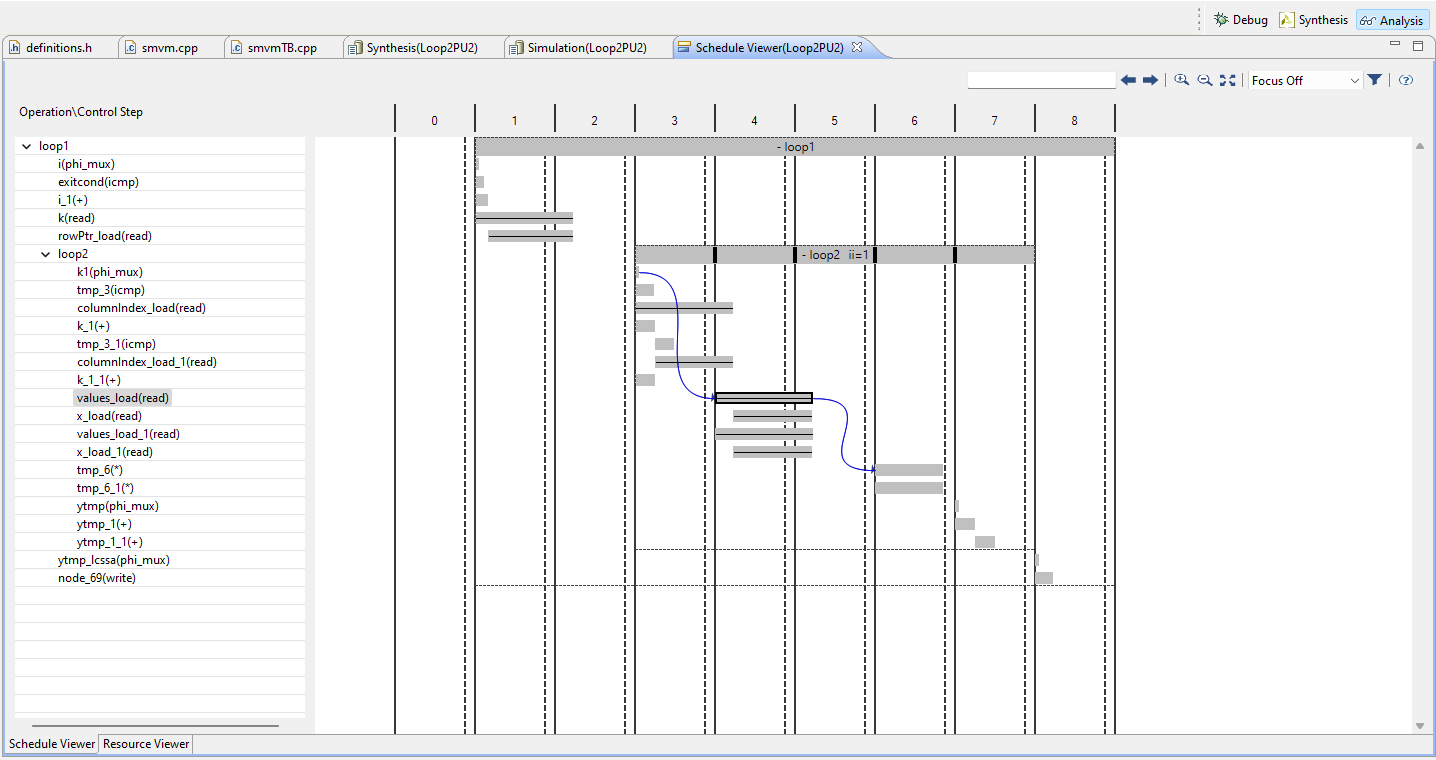
\includegraphics[width=1\textwidth]{solutions/s5/s5analysis.png}
	\caption{HLS Solution 5 Analysis}
\end{figure}

\begin{table}[H]
	\centering
	\begin{tabular}{|l|c|c|c|c|}
		\hline
		\textbf{Name}    & \textbf{BRAM\_18K} & \textbf{DSP48E} & \textbf{FF} & \textbf{LUT} \\ \hline
		DSP              & -                   & -               & -           & -            \\ 
		Expression       & -                   & 6              & 0           & 257          \\ 
		FIFO             & -                   & -               & -           & -            \\ 
		Instance         & -                   & -               & -           & -            \\ 
		Memory           & 0                   & -               & -          & -            \\ 
		Multiplexer      & -                   & -               & -           & 78          \\ 
		Register         & -                   & -               & 597         & 64            \\ \hline
		\textbf{Total}   & 0                   & 6               & 597         & 399          \\ \hline
		\textbf{Available} & 280               & 220             & 106400      & 53200        \\ \hline
		\textbf{Utilization (\%)} & 0            & 2               & $\sim$0     & $\sim$0      \\ \hline
	\end{tabular}
	\caption{HLS Solution 5 Utilization Estimates Summary}
	\label{tab:hls-solution-5-utilization-estimates-summary}
\end{table}

\begin{table}[H]
	\centering
	\begin{tabular}{|c|c|c|c|c|c|c|c|}
		\hline
		\multicolumn{1}{|c|}{RTL} & \multicolumn{1}{|c|}{Status} & \multicolumn{3}{c|}{\textbf{Latency}} & \multicolumn{3}{c|}{\textbf{Interval}} \\
		&  & min & avg & max & min & avg & max \\
		\hline
		VHDL & Pass & 37 & 37 & 37 & NA & NA & NA \\
		\hline
	\end{tabular}
	\caption{HLS Solution 5 C/RTL Cosimulation Summary }
	\label{tab:hls-solution-5-cosimulation-summary}
\end{table}

Si può notare, rispetto alla soluzione hardware 2, un aumento dell'utilizzazione delle risorse del $60\%$ per quanto riguarda le LUT e di circa il $41\%$ per quanto riguarda i FF. Inoltre, si può evidenziare come il numero dei DSP sia raddoppiato.

\begin{table}[H]
	\centering
	\begin{minipage}[t]{0.45\linewidth}
		\centering
		\begin{tabular}{|l|r|}
			\hline
			\textbf{Resource} & \textbf{VHDL} \\
			\hline
			SLICE & 69 \\
			\hline
			LUT & 184 \\
			\hline
			FF & 196 \\
			\hline
			DSP & 6 \\
			\hline
			BRAM & 0 \\
			\hline
			SRL & 0 \\
			\hline
		\end{tabular}
		\caption{HLS Solution 5 Export RTL Resource Usage}
		\label{tab:hls-solution-5-export-rtl-resoruce-usage}
	\end{minipage}
	\hfill
	\begin{minipage}[t]{0.45\linewidth}
		\centering
		\begin{tabular}{|l|r|}
			\hline
			\textbf{Timing} & \textbf{VHDL} \\
			\hline
			CP required & 10.000 \\
			\hline
			CP achieved post-synthesis & 7.927 \\
			\hline
			CP achieved post-implementation & 7.465 \\
			\hline
		\end{tabular}
		\caption{HLS Solution 5 Export RTL Final Timing}
		\label{tab:hls-solution-5-export-rtl-final-timing}
	\end{minipage}
\end{table}